\documentclass[tikz,border=3pt]{standalone}
\usepackage{tikz}
\usetikzlibrary{arrows.meta,positioning,fit,calc}
\begin{document}
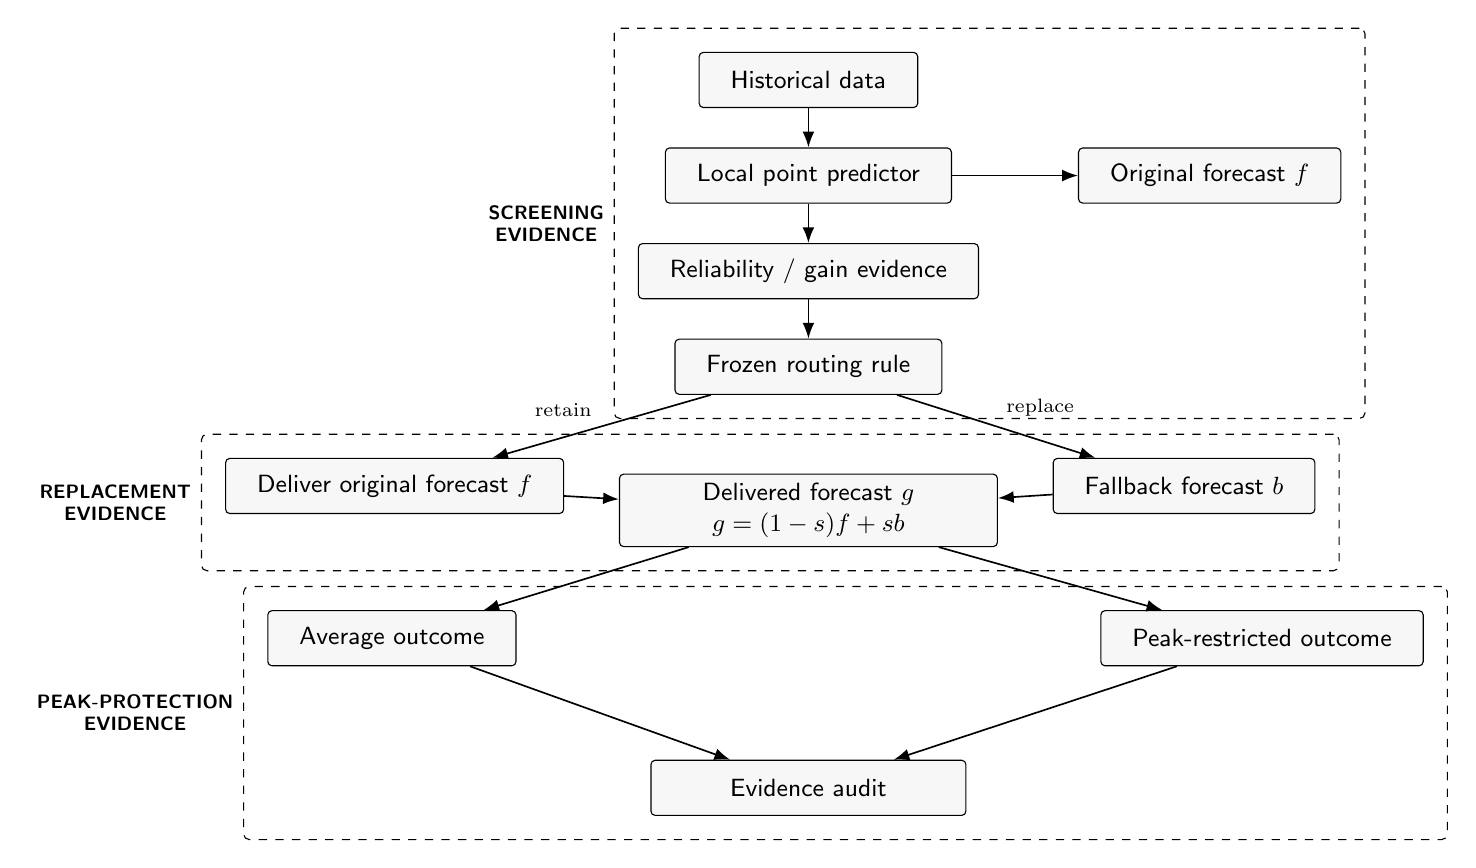
\begin{tikzpicture}[
  font=\sffamily\small,
  box/.style={draw,rounded corners=1.5pt,minimum height=7mm,align=center,inner xsep=4mm,fill=gray!6},
  arrow/.style={-{Latex[length=2mm]},semithick},
  group/.style={draw,rounded corners=2pt,dashed,inner sep=3mm},
  lab/.style={font=\sffamily\bfseries\scriptsize,align=center}
]
\node[box] (hist) {Historical data};
\node[box,below=5mm of hist] (point) {Local point predictor};
\node[box,right=16mm of point] (orig) {Original forecast $f$};
\node[box,below=5mm of point] (evid) {Reliability / gain evidence};
\node[box,below=5mm of evid] (rule) {Frozen routing rule};
\node[box,below left=8mm and 14mm of rule] (keep) {Deliver original forecast $f$};
\node[box,below right=8mm and 14mm of rule] (fallback) {Fallback forecast $b$};
\node[box,below=10mm of rule,minimum width=48mm] (deliv) {Delivered forecast $g$\\$g=(1-s)f+sb$};
\node[box,below left=8mm and 13mm of deliv] (avg) {Average outcome};
\node[box,below right=8mm and 13mm of deliv] (peak) {Peak-restricted outcome};
\node[box,below=9mm of deliv, yshift=-18mm, minimum width=40mm] (audit) {Evidence audit};

\draw[arrow] (hist) -- (point);
\draw[arrow] (point) -- (orig);
\draw[arrow] (point) -- (evid);
\draw[arrow] (evid) -- (rule);
\draw[arrow] (rule) -- node[above left,font=\scriptsize]{retain} (keep);
\draw[arrow] (rule) -- node[above right,font=\scriptsize]{replace} (fallback);
\draw[arrow] (keep) -- (deliv);
\draw[arrow] (fallback) -- (deliv);
\draw[arrow] (deliv) -- (avg);
\draw[arrow] (deliv) -- (peak);
\draw[arrow] (avg) -- (audit);
\draw[arrow] (peak) -- (audit);

\node[group,fit=(hist)(point)(orig)(evid)(rule),label={[lab]left:SCREENING\\EVIDENCE}] {};
\node[group,fit=(keep)(fallback)(deliv),label={[lab]left:REPLACEMENT\\EVIDENCE}] {};
\node[group,fit=(avg)(peak)(audit),label={[lab]left:PEAK-PROTECTION\\EVIDENCE}] {};
\end{tikzpicture}
\end{document}
